\documentclass[12pt,a4paper,article,english,firamath]{nsi}
\pagestyle{empty}
\usepackage{fontawesome5}
\begin{document}
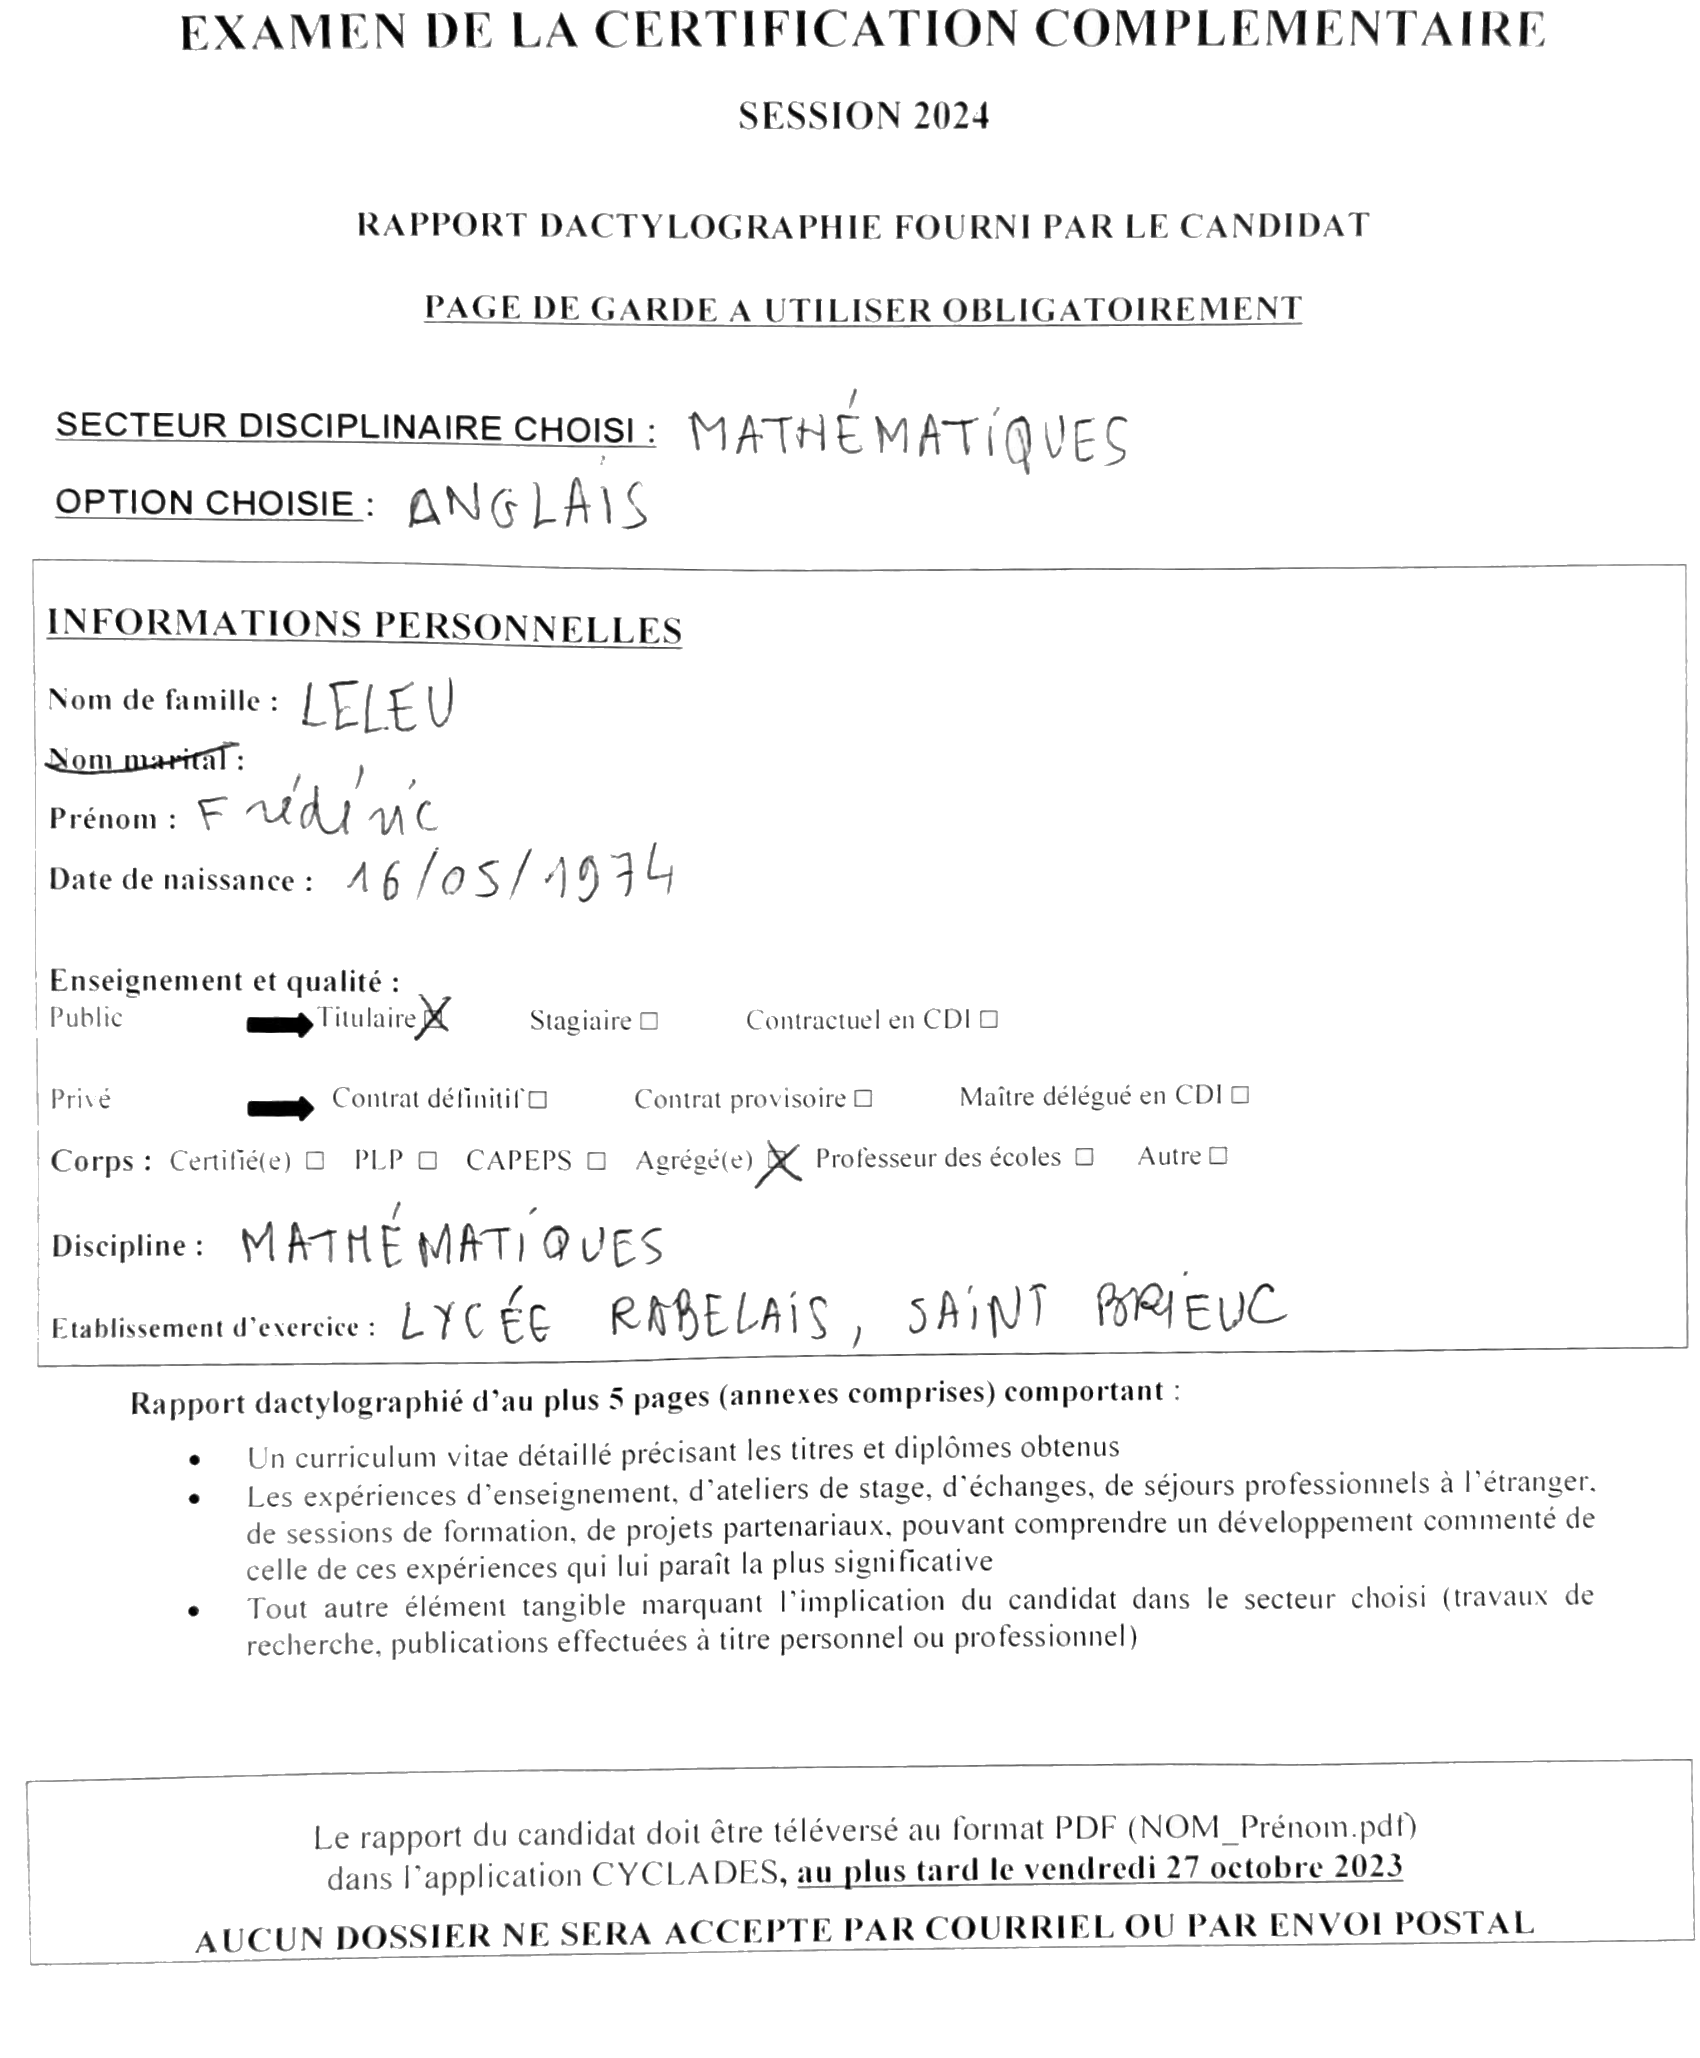
\includegraphics[width=17cm]{img/garde.png}
\newpage
{\Large\titlefont FRÉDÉRIC LELEU}\\
{\color{UGLiBlue}\textbf{Mathematics and Computer Science Teacher}}\\

{\color{UGLiBlue}\faEnvelope} 29, avenue d'Armorique, 22000 Saint Brieuc\\
{\color{UGLiBlue}\faAt} frederic.leleu@ac-rennes.fr\\
{\color{UGLiBlue}\faPhone*} 06 99 13 08 41\\

%{\color{UGLiBlue}\faCalendar*}


\begin{multicols}{2}
{\color{UGLiBlue}\large\titlefont TEACHING EXPERIENCE\\[-1em]\hrule}

\bigskip Teaching Assistant \\
{\color{UGLiBlue}\textbf{EPITA }}\\
{\color{lightgray}\faCalendar*  1998 - 2000\\ \faMapMarker* Paris-Villejuif (94)}

\bigskip Math teacher \\
{\color{UGLiBlue}\textbf{Éducation Nationale}}\\
{\color{lightgray}\faCalendar*  2000 - Present\\ \faMapMarker*\small Argenteuil (95), Ermont (95), Saint Brieuc (22)}

\bigskip CS teacher \\
{\color{UGLiBlue}\textbf{Éducation Nationale}}\\
{\color{lightgray}\faCalendar*  2013 - Present\\ \faMapMarker* Ermont (95), Saint Brieuc (22)}

\bigskip Python Trainer \\
{\color{UGLiBlue}\textbf{Académie de Rennes}}\\
{\color{lightgray}\faCalendar*  2017 - 2018\\ \faMapMarker* Rennes (35)}

\bigskip CS Teacher / Educator \\
{\color{UGLiBlue}\textbf{INSPÉ de Bretagne}}\\
{\color{lightgray}\faCalendar*  2022 - 2023\\ \faMapMarker* Rennes (35)}



\columnbreak
{\color{UGLiBlue}\large\titlefont EDUCATION\\[-1em]\hrule}


\bigskip Maîtrise de Mathématiques Pures \\
{\color{UGLiBlue}\textbf{Université Pierre et Marie Curie Paris 6}}\\
{\color{lightgray}\faCalendar*  1996\\ \faMapMarker* Paris (75)}

\bigskip CAPES de Mathématiques \\
{\color{UGLiBlue}\textbf{Université Pierre et Marie Curie Paris 6}}\\
{\color{lightgray}\faCalendar*  2000\\ \faMapMarker* Paris (75)}

\bigskip Agrégation de Mathématiques \\
{\color{UGLiBlue}\textbf{Université Paris-Saclay}}\\
{\color{lightgray}\faCalendar*  2009\\ \faMapMarker* Orsay (91)}

\bigskip DIU Formation à la Science Informatique - ISN \\
{\color{UGLiBlue}\textbf{Université Versailles Saint-Quentin}}\\
{\color{lightgray}\faCalendar*  1996\\ \faMapMarker* Versailles (78)}

\bigskip Enseigner l'informatique au lycée \\
{\color{UGLiBlue}\textbf{Université Rennes 2}}\\
{\color{lightgray}\faCalendar*  2020\\ \faMapMarker* Rennes (35)}

\end{multicols}
\ \\
\begin{multicols}{2}
{\color{UGLiBlue}\large\titlefont LANGUAGES\\[-1em]\hrule}
\medskip 
French: Native Speaker\\
English : Level C1\\
Spanish : Level B2\\
Slovak : Level A2\\

\columnbreak

{\color{UGLiBlue}\large\titlefont INTERESTS\\[-1em]\hrule}
\medskip 
Programming, Music, Reading (mainly in English)

\end{multicols}
\newpage
I started teaching mathematics almost 25 years ago, but I've been programming on a daily basis since I was 13.\\
15 years ago or so, I decided to explain to my math students how a sorting algorithm works (maybe I was getting a bit bored of teaching the same math again and again, and never getting any question back from my pupils). I was amazed by the way they reacted to the class : they seemed much more focused than usual and teemed with numerous questions, each one more interesting than the other.\\
So when ISN was created I embraced the opportunity with a lot of enthusiasm and now that NSI is here to stay I spend most of my time teaching computer science. Officially, I'm still teaching "Mathématiques pour l'Informatique" in BTS SIO, but I try to colorate this math teaching as much as I can with Computer Science and I like to think that most of my students are grateful for this.\\

This year I started teaching mathematics in English (acting as a substitute for a colleague who has health issues) and until now it has been a pleasant, rewarding experience. You will find below an example of what I'm actually doing, which I'll be glad to explain.\\
Right now, my main concern is that I'm not yet able to gauge my pupils' level in English. I obviously try to speak as much English as possible but sometimes, I guess It would be better to explain some aspects of the problem we're trying to solve in French.\\

However, the main reason that pushes me to get this certification is Computer Science. Indeed, it abounds with technical terms, most of which are in English, so when teaching I constantly find myself switching from French to English, then back to French and so on. With this certification I could offer my students the possibility to have a whole lesson in English (which is in my opinion a really good option considering the way technique and English are intertwined when it comes to Computer Science). I consider myself lucky : when my pupils are working with computers, their group is split in two. As I'm sure at least half of them would like to try a whole class in English maybe we could dedicate one of the  subgroups to this.

\newpage 
\titre{Secret Santa\ \scriptsize(solution)}
\classe{Euro 1\ere}
\maketitle
watch the video here : {\color{UGLiBlue} \texttt{https://video.toutatice.fr/video/41820-secret-santa/}}
\subsubsection*{From 00:00 to 00:42}
Explain what is Secret Santa.
\begin{encadrecolore}{Answer}{UGLiRed}
    Secret Santa is a method which makes each person in a group choose another one to give a present to, so that everybody buys a present for someone and also gets one.
\end{encadrecolore}
\subsubsection*{From 01:22 to 01:36}
What are the two fundamental things for a perfect Secret Santa ?
\begin{encadrecolore}{Answer}{UGLiRed}
    \begin{enumerate}
        \item It should be anonymous : nobody should know who bought his or her present.
        \item It should be perfectly random : you should have the same probability of getting a present from each member of the group.
    \end{enumerate}
\end{encadrecolore}
\subsubsection*{From 01:44 to 02:03}
How does Hannah describe the "hat method" ?
\begin{encadrecolore}{Answer}{UGLiRed}
    Everybody writes his or her name on a piece of paper and puts it in a hat.
    Then each member of the group successively picks a paper and reads a name. If someone picks his or her own name, he or she puts the paper back in the hat, otherwise, he or she will have to offer a present to the person whose name's written on the paper.
\end{encadrecolore}
\subsubsection*{From 02:03 to 02:46}
What is the obvious problem with this method and what does the group have to do in this case ?
\begin{encadrecolore}{Answer}{UGLiRed}
    If the last person's left with his or her own paper, there's nothing to do but start over.
\end{encadrecolore}
Why is there also an anonymity violation if the person before the last one pulls his or her name ?
\begin{encadrecolore}{Answer}{UGLiRed}
    Because in this case, he or she must take the only other remaining paper and everybody knows that the last person will get his or hers.
\end{encadrecolore}
\subsubsection*{From 02:46 to 10:59}
\picright{0.25}{img/tree_santa3_sol}{
    Despite of anonymity issues, let's see how  Secret Santa works with 3 persons.\\

    Complete this probability tree.\\

    When the method works, can we say is it completely random ?\\
    Justify your answer.}

\begin{encadrecolore}{Answer}{UGLiRed}
    No it is not, because for example, when the method works A it twice likely to buy for C than for B.
\end{encadrecolore}
\subsubsection*{From 11:00 till the end}
Explain what's the right way to organize a Secret Santa.
\begin{encadrecolore}{Answer}{UGLiRed}
\begin{itemize}
    \item Take as many cards as the number of people and write "You are number i" at the top and "You are buying for i" the bottom of each ($i$ starting from one to $n$, $n$ being the number of people). 
    \item Lay them face down and shuffle them.
    \item Cut them all up in the middle.
    \item Shift the tops along by one.
    \item Everybody take the two corresponding parts and find what's his or her number and who he or she is buying for.
\end{itemize}
\end{encadrecolore}
\subsection*{Bonus}

What's a derangement ?
\begin{encadrecolore}{Answer}{UGLiRed}
    A derangement is a permutation in which no object retains its original position.
\end{encadrecolore}

Complete the following tree for a "hat method" with 4 person.
\begin{center}
    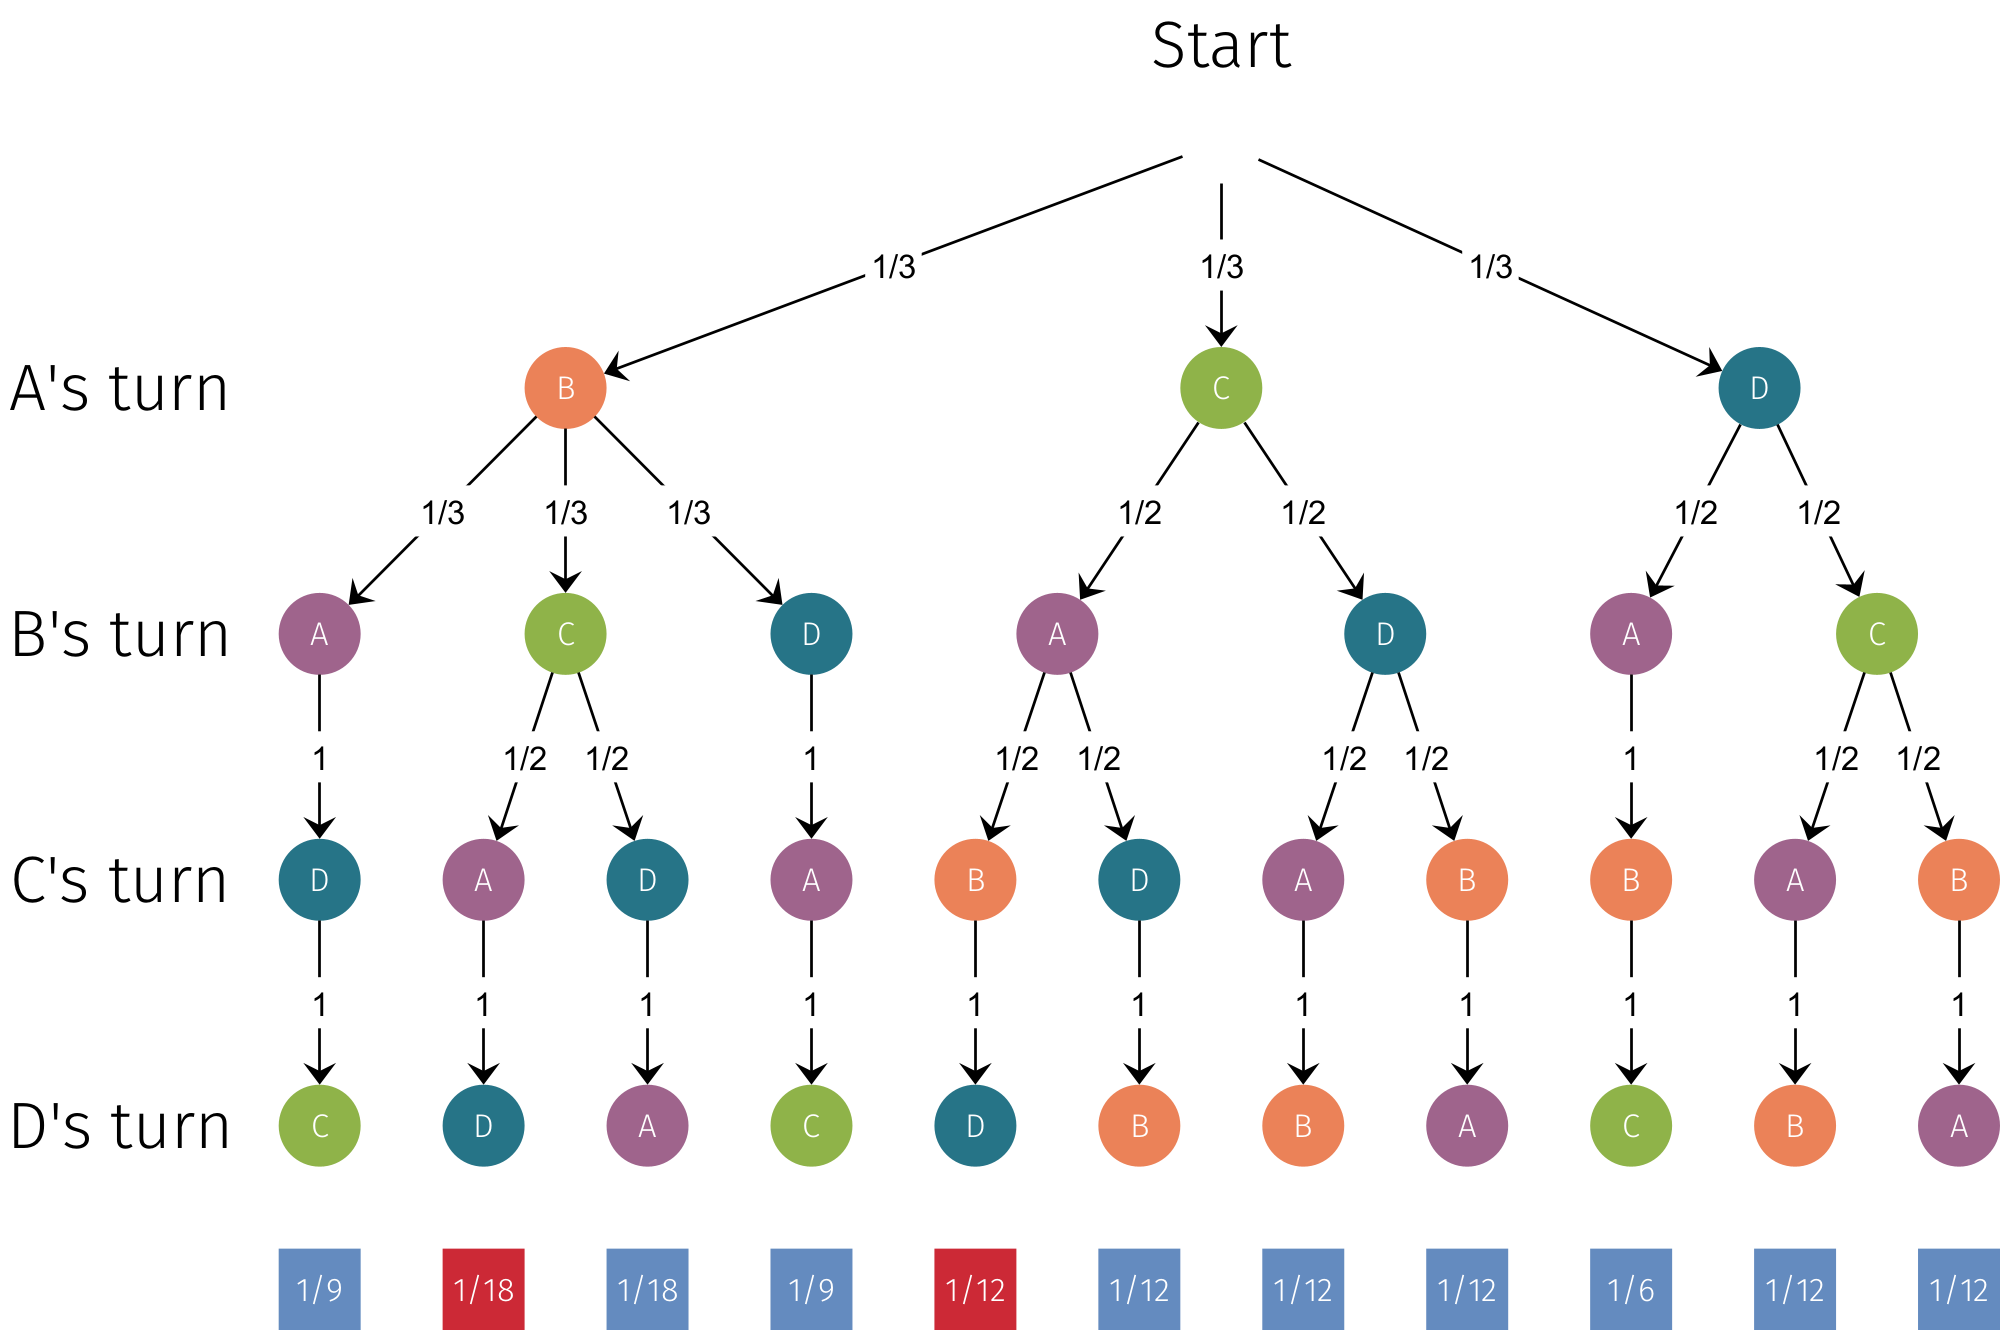
\includegraphics[width=13cm]{img/tree_santa4_sol.png}
\end{center}
What's the probability of a failure ?
\begin{encadrecolore}{Answer}{UGLiRed}
    It is $\frac{1}{18}+\frac{1}{12}=\frac{5}{36}\simeq 8.33\%$.
\end{encadrecolore}

\end{document}